\documentclass{report}

\usepackage[T1]{fontenc}
\usepackage[utf8]{inputenc}
\usepackage[brazilian]{babel}
\usepackage{graphicx}
\usepackage[export]{adjustbox}[2011/08/13]
\usepackage{float}
\usepackage[pdftex]{hyperref}
\usepackage{epstopdf}
\usepackage{etoolbox}
\usepackage{amsmath}
\usepackage{amsfonts}
\usepackage{amssymb}
\usepackage{caption}
\usepackage{subcaption}
\usepackage{setspace}
\usepackage{tikz}
\usepackage{listings}
\usepackage{xcolor} 

\bibliographystyle{eric}
\patchcmd{\thebibliography}{\section*}{\section}{}{}


\newcommand{\R}{\ensuremath{\mathbb{R}}}
\newcommand{\Prob}{\ensuremath{\mathbb{P}}}
\newcommand{\K}{\ensuremath{\mathbb{K}}}
\newcommand{\U}{\ensuremath{\mathbb{U}}}
\newcommand{\N}{\ensuremath{\mathbb{N}}}
\newcommand{\Lg}{\ensuremath{\mathbb{L}}}
\newcommand{\T}{\ensuremath{\rm Tr}}
\newcommand{\sg}{{\sigma(x_k)}}

\newcommand{\G}{\ensuremath{\mathcal{G}}}
\newcommand{\F}{\ensuremath{\mathcal{F}}}
\newcommand{\C}{\ensuremath{\mathcal{C}}}
\newcommand{\E}{\ensuremath{\mathcal{E}}}
\newcommand{\Hn}{\ensuremath{\mathcal{H}}}
\newcommand{\Hoo}{\ensuremath{\mathcal{H}_\infty}}
\newcommand{\Hop}{\ensuremath{\mathcal{H}_{op}}}
% --------------------------------------------------
\newtheorem{theo}{Teorema}
\newtheorem{exa}{Exemplo}
\newtheorem{lemm}{Lema}
\newtheorem{coro}{Corolário}
\newtheorem{defn}{Definição}[section]

\begin{document}

\begin{titlepage}
\begin{center}

\newcommand{\HRule}{\rule{\linewidth}{0.5mm}}
% Upper part of the page. The '~' is needed because \\
% only works if a paragraph has started.

\includegraphics[width=0.15\textwidth]{logoUnicamp}~\\[1cm]

\textsc{\LARGE Universidade Estadual de Campinas}\\[1.5cm]

\textsc{\Large Faculdade de Engenharia Mecânica}\\[0.5cm]

% Title
\HRule \\[0.4cm]
{ \huge \bfseries ES664 - Laboratório de Eletrônica para Automação Industrial\\ \vspace{1cm} Relatório - Experimento 4\\
\Large{Acionamento de motor DC} \\[0.4cm] }

\HRule \\[1.5cm]

% Author and supervisor
\begin{minipage}{0.6\textwidth}
\begin{flushleft} \large
\emph{Nome:}\\
Daniel Dello Russo Oliveira\\Marcelli Tiemi Kian
\end{flushleft}
\end{minipage}
\begin{minipage}{0.2\textwidth}
\begin{flushright} \large
\emph{RA}\\ 101918\\117892
\end{flushright}
\end{minipage}

\vfill

% Bottom of the page
{\large \today}

\end{center}
\end{titlepage}


\onehalfspacing
\section{Objetivos}
	Essa simulação tem como objetivo a familiarização com o ambiente de Simulink, com a toolbox SimPowerSystems e com retificadores não controlados.
	 
\section{Retificador monofásico}
Através do Simulink implementamos o retificador monofásico de onda completa detalhado em \cite{bb:roteirosim1} conforme mostrado na figura \ref{fig:msim}.
\begin{figure}[H]
	\centering
	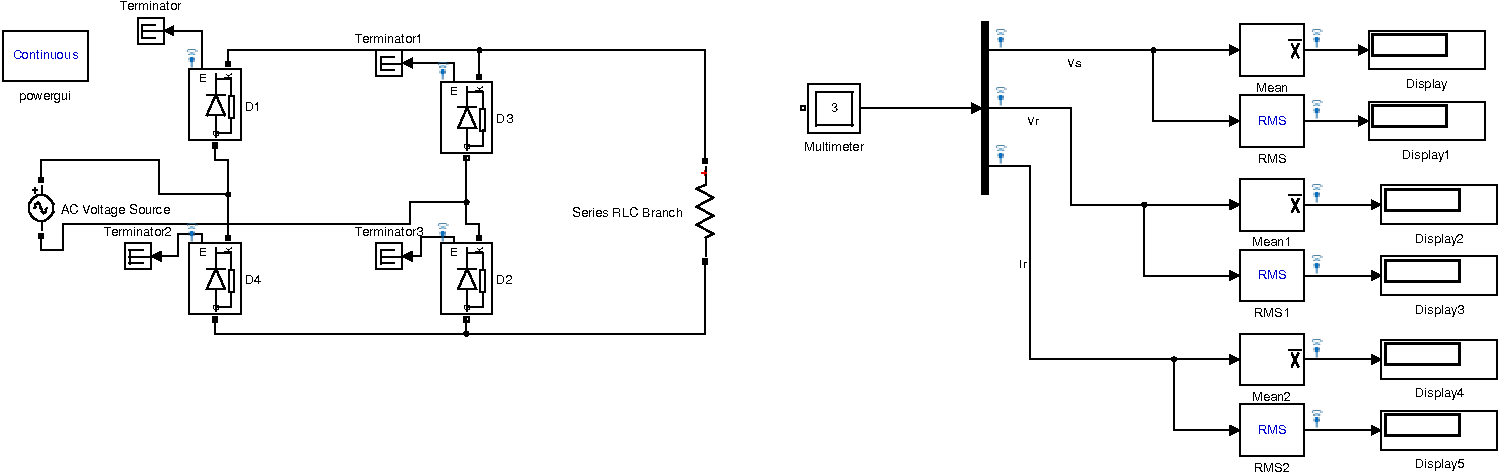
\includegraphics[width=\linewidth]{matlab/mono_sim}
	\caption{Esquema para simulação do retificador monofásico}
	\label{fig:msim}
\end{figure}

Extraímos dessa simulação as curvas de tensão na fonte (figura \ref{fig:mvs}), tensão na carga (figura \ref{fig:mvr}) e corrente na carga (figura \ref{fig:mir}) para dois períodos da fonte.
\begin{figure}[H]
	\centering
	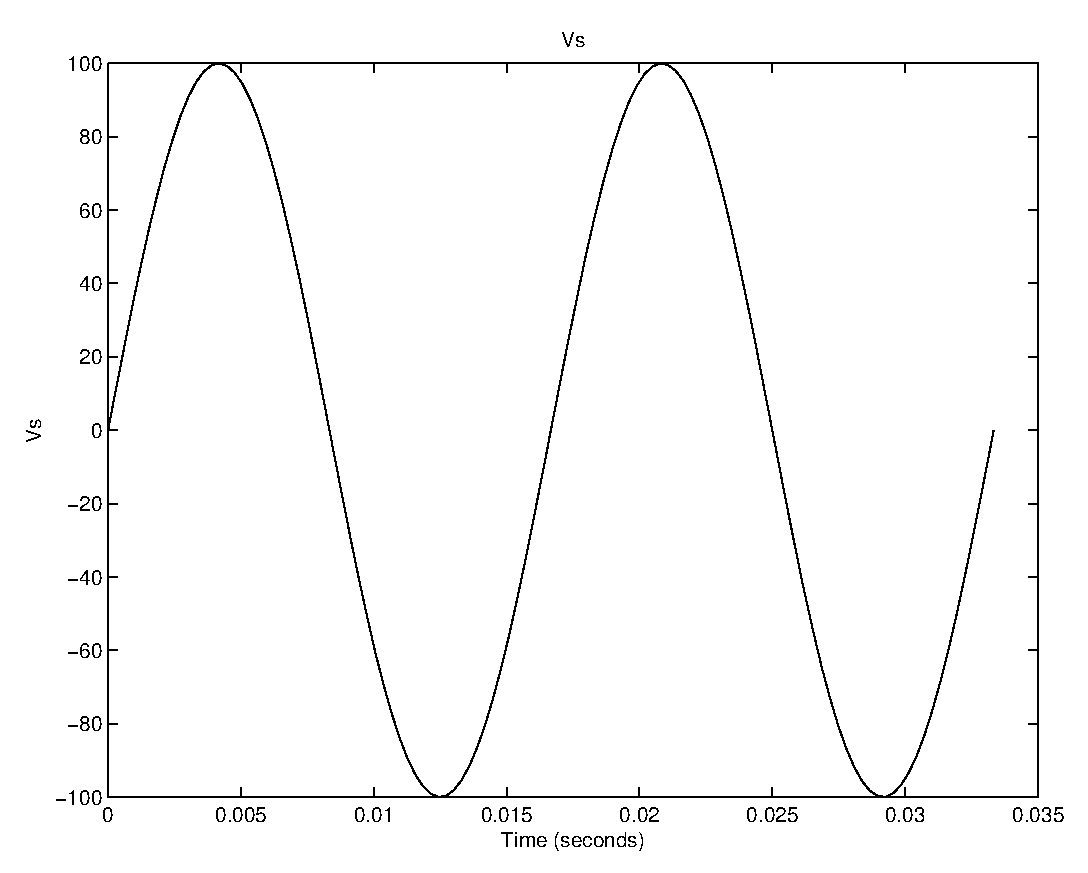
\includegraphics[width=0.7\linewidth]{matlab/mono_vs}
	\caption{Tensão da fonte para retificador monofásico}
	\label{fig:mvs}
\end{figure}
\begin{figure}[H]
	\centering
	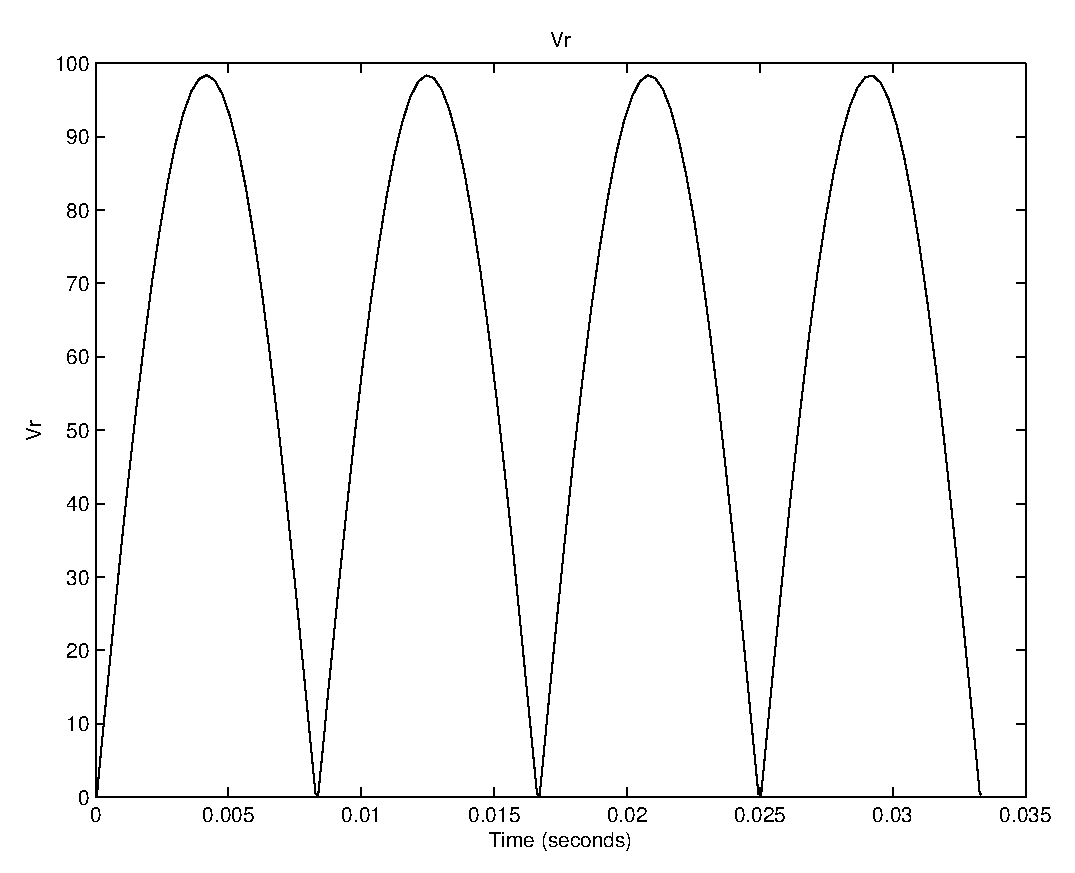
\includegraphics[width=0.7\linewidth]{matlab/mono_vr}
	\caption{Tensão na carga para retificador monofásico}
	\label{fig:mvr}
\end{figure}
\begin{figure}[H]
	\centering
	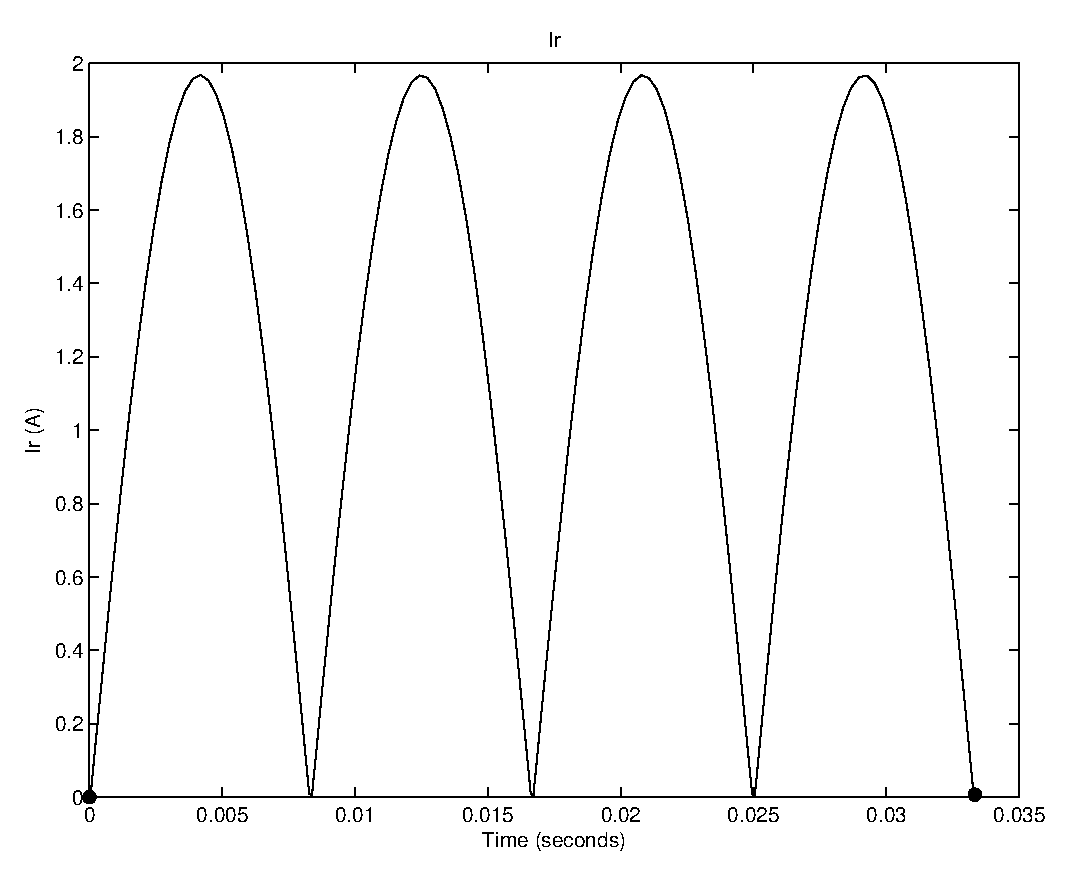
\includegraphics[width=0.7\linewidth]{matlab/mono_ir}
	\caption{Corrente na carga para retificador monofásico}
	\label{fig:mir}
\end{figure}

Medimos as tensões e correntes médias e efetivas na carga, obtendo os seguintes valores:
\begin{equation}
\overline{Vr} = 62.0713\ V
\end{equation}
\begin{equation}
\overline{Ir} = 1.2414\ A
\end{equation}
\begin{equation}
Vr_{rms} =  69.2708\ V
\end{equation}
\begin{equation}
Ir_{rms} = 1.3854\ A
\end{equation}

Obtivemos também as curvas de tensão e corrente para cada diodo do arranjo, representadas nas figuras \ref{fig:md1}, \ref{fig:md2}, \ref{fig:md3} e \ref{fig:md4}
\foreach \n in {1,...,4}{
	\begin{figure}[H]
		\centering
		\begin{subfigure}[b]{0.4\linewidth}
			\includegraphics[width=\linewidth]{matlab/mono_d\n i}
			\caption{Corrente no diodo}
			\label{fig:md\n i}
		\end{subfigure}
		\begin{subfigure}[b]{0.4\linewidth}
			\centering
			\includegraphics[width=\linewidth]{matlab/mono_d\n v}
			\caption{Tensão no diodo}
			\label{fig:md\n v}
		\end{subfigure}
		\caption{Curvas do diodo \n\ para retificador monofásico}
		\label{fig:md\n}
	\end{figure}
}

Conforme podemos ver analisando as curvas dos diodos (figuras \ref{fig:md1}, \ref{fig:md2}, \ref{fig:md3} e \ref{fig:md4}) e a tensão da fonte (figura \ref{fig:mvs}), para uma carga puramente resistiva, durante o semi-ciclo positivo da fonte, os diodos 1 e 2 estão conduzindo enquanto 3 e 4 estão bloqueando, dessa forma a tensão sobre a carga é $Vs$. Já no semi-ciclo negativo da fonte, os diodos 3 e 4 estão conduzindo enquanto 1 e 2 estão bloqueando, fazendo que a tensão na carga seja de $-Vs$. Dessa forma conseguímos transformar uma tensão senoidal sobre a carga em uma tensão sempre positiva, de maneira que seu valor médio não seja nulo.
Podemos calcular a tensão média teórica sobre a carga através da equação \ref{eq:mmean}
\begin{equation}
	\overline{Vr} = \frac{1}{\pi} \int_{0}^{\pi}{Vs sin(\theta)d\theta} = \frac{2 Vs}{\pi}
	\label{eq:mmean}
\end{equation}
Para calcular o valor efetivo da tensão sobre a carga utilizamos a equação \ref{eq:mrms}.
\begin{equation}
	Vr_{rms} = \sqrt{\frac{1}{\pi} \int_{0}^{\pi}{(Vs sin(\theta))^2 d\theta}} = \frac{Vs}{\sqrt{2}}
	\label{eq:mrms}
\end{equation}
Utilizando os valores da simulação ($Vs\ =\ 100\ V$), encontramos as tensões e correntes esperadas:
\begin{equation}
\overline{Vr} = 63.6620\ V
\end{equation}
\begin{equation}
\overline{Ir} = 1.2732\ A
\end{equation}
\begin{equation}
Vr_{rms} =  70.7107\ V
\end{equation}
\begin{equation}
Ir_{rms} = 1.4142\ A
\end{equation}
Conforme podemos ver os valores medidos e esperados diferem levemente, isso se deve às imprecisões numéricas da simulação, à queda de tensão introduzida pelos diodos, ao pequeno período de amostragem, entre outros fatores.

Calculamos o fator de retificação teórico (\ref{eq:mrft}) e medido ({\ref{eq:mrfm}) usando a equação \ref{eq:rf}.
\begin{equation}
	\sigma = \frac{\overline{P}}{P_{rms}} = \frac{\overline{Vr}^2}{Vr_{rms}^2}
	\label{eq:rf}
\end{equation}

\begin{equation}
	\sigma_t = 0.8106
	\label{eq:mrft}
\end{equation}
\begin{equation}
	\sigma_m = 0.8029
	\label{eq:mrfm}
\end{equation}

Encontramos por fim o fator de forma teórico (\ref{eq:mfft}) e medido ({\ref{eq:mffm}) usando a equação \ref{eq:ff}.
\begin{equation}
FF = \frac{\overline{Vr}}{Vr_{rms}}
\label{eq:ff}
\end{equation}

\begin{equation}
FF_t = 1.1107
\label{eq:mfft}
\end{equation}
\begin{equation}
FF_m = 1.1160
\label{eq:mffm}
\end{equation}
\section{Retificador trifásico}
Através do Simulink implementamos o retificador trifásico de onda completa detalhado em \cite{bb:roteirosim1} conforme mostrado na figura \ref{fig:tsim}.
\begin{figure}[H]
	\centering
	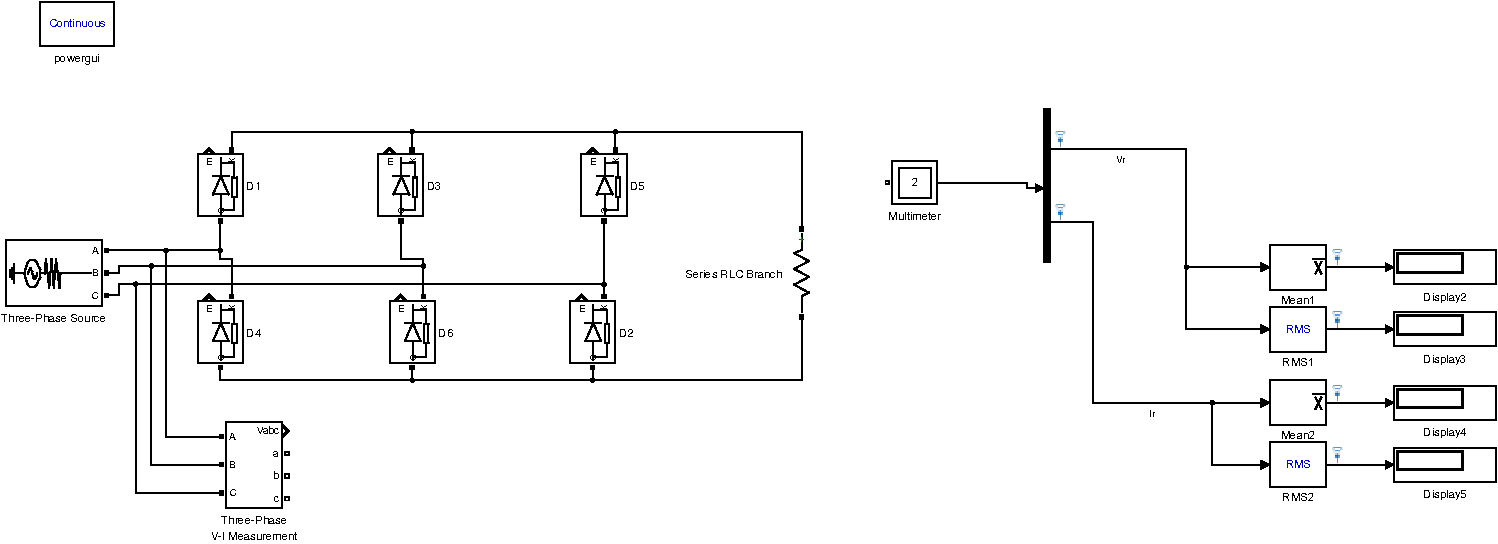
\includegraphics[width=\linewidth]{matlab/tri_sim}
	\caption{Esquema para simulação do retificador trifásico}
	\label{fig:tsim}
\end{figure}

Extraímos dessa simulação as curvas das tensões de fase na fonte trifásica (figura \ref{fig:tvs}), da tensão na carga (figura \ref{fig:tvr}) e da corrente na carga (figura \ref{fig:tir}) para dois períodos da fonte.
\begin{figure}[H]
	\centering
	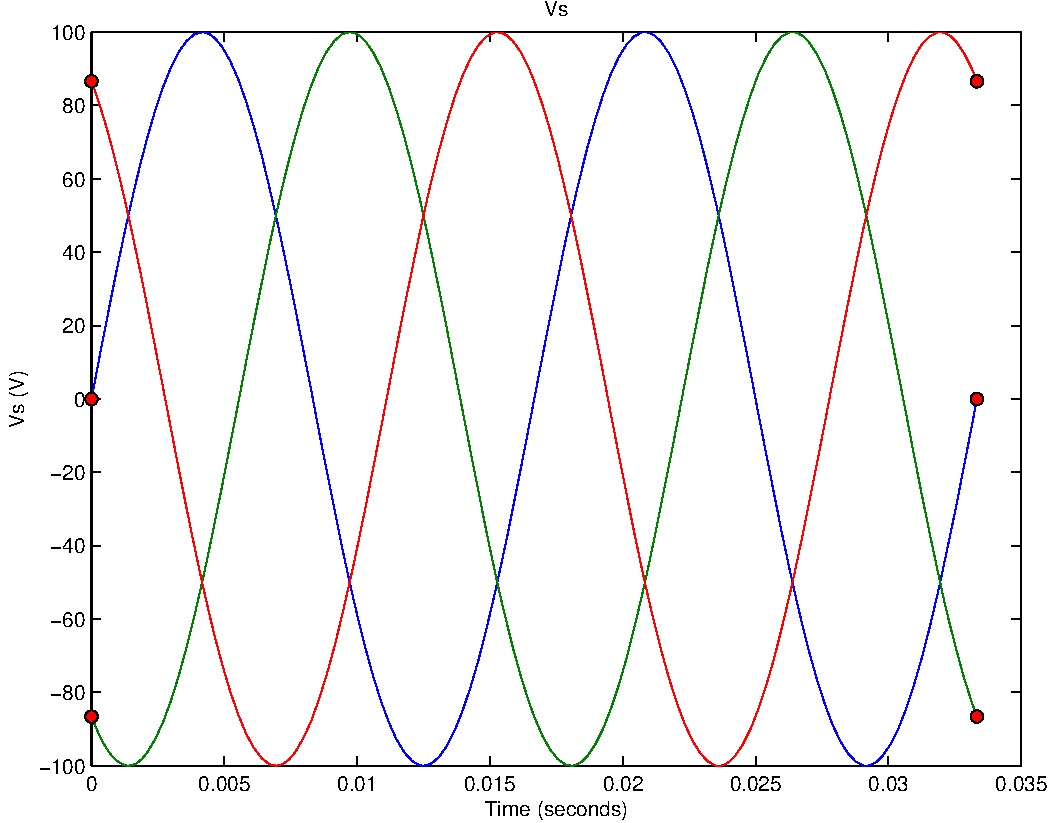
\includegraphics[width=0.7\linewidth]{matlab/tri_vs}
	\caption{Tensões das fontes para retificador trifásico}
	\label{fig:tvs}
\end{figure}
\begin{figure}[H]
	\centering
	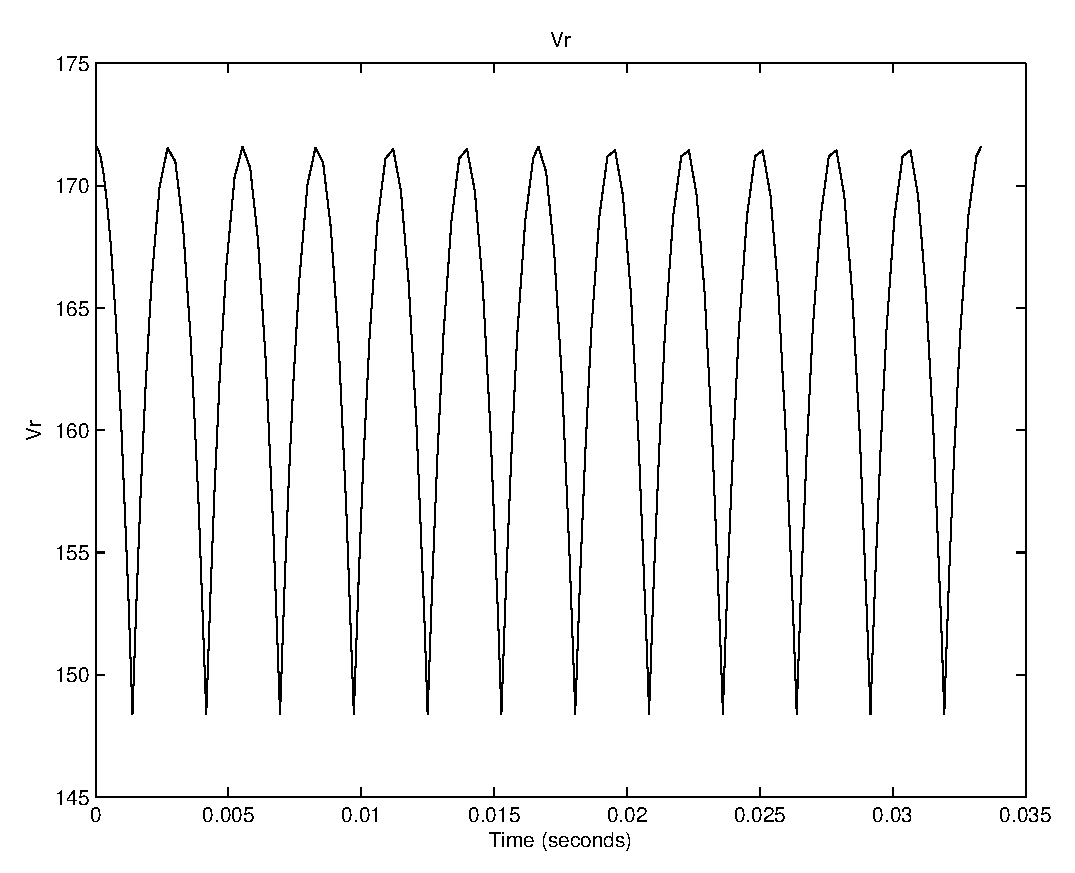
\includegraphics[width=0.7\linewidth]{matlab/tri_vr}
	\caption{Tensão na carga para retificador trifásico}
	\label{fig:tvr}
\end{figure}
\begin{figure}[H]
	\centering
	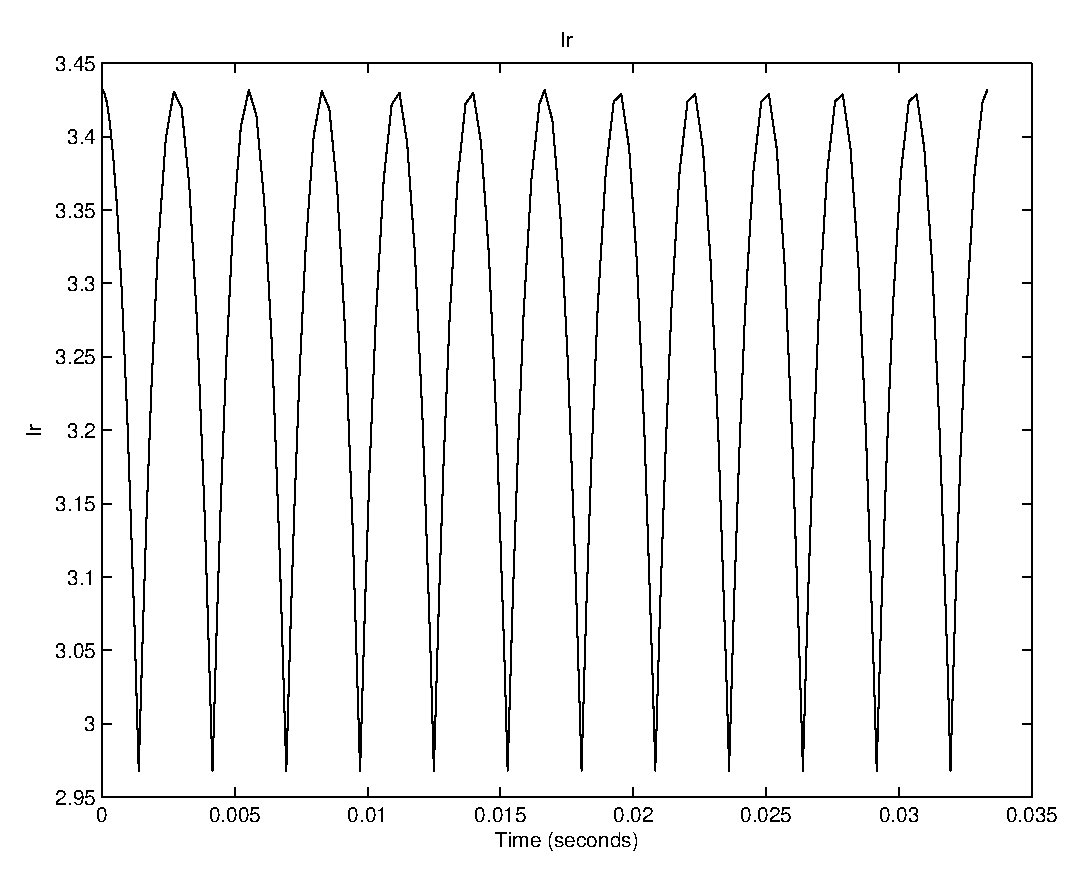
\includegraphics[width=0.7\linewidth]{matlab/tri_ir}
	\caption{Corrente na carga para retificador trifásico}
	\label{fig:tir}
\end{figure}

Medimos as tensões e correntes médias e efetivas na carga, obtendo os seguintes valores:
\begin{equation}
\overline{Vr} = 163.7921\ V
\end{equation}
\begin{equation}
\overline{Ir} = 3.2758\ A
\end{equation}
\begin{equation}
Vr_{rms} =  163.9391\ V
\end{equation}
\begin{equation}
Ir_{rms} = 3.2788\ A
\end{equation}

Obtivemos também as curvas de tensão e corrente para cada diodo do arranjo, representadas nas figuras \ref{fig:td1}, \ref{fig:td2}, \ref{fig:td3}, \ref{fig:td4}, \ref{fig:td5} e \ref{fig:td6}

\foreach \n in {1,...,6}{
	\begin{figure}[H]
		\centering
		\begin{subfigure}[b]{0.4\linewidth}
			\includegraphics[width=\linewidth]{matlab/tri_d\n i}
			\caption{Corrente no diodo}
			\label{fig:td\n i}
		\end{subfigure}
		\begin{subfigure}[b]{0.4\linewidth}
			\centering
			\includegraphics[width=\linewidth]{matlab/tri_d\n v}
			\caption{Tensão no diodo}
			\label{fig:td\n v}
		\end{subfigure}
		\caption{Curvas do diodo \n\ para retificador trifásico}
		\label{fig:td\n}
	\end{figure}
}

Conforme podemos ver analisando as curvas dos diodos (figuras \ref{fig:td1}, \ref{fig:td2}, \ref{fig:td3}, \ref{fig:td4}, \ref{fig:td5} e \ref{fig:td6}) e a tensão da fonte (figura \ref{fig:tvs}), para uma carga puramente resistiva, quando a tensão da fonte A é a maior e a tensão da fonte C é a menor os diodos 1 e 2 estão conduzindo e os outros bloqueando, uma vez que a tensão da fonte B ultrapassa a de A, os diodos 2 e 3 passam a conduzir, quando a fonte C ultrapassa A por sua vez, temos os diodos 3 e 4 conduzindo e assim sucessivamente.

Podemos calcular a tensão média teórica sobre a carga através da equação \ref{eq:tmean}.
\begin{equation}
\overline{Vr} = \frac{3}{\pi} \int_{\frac{\pi}{6}}^{\frac{4\pi}{6}}{Vs(sin(\theta) - sin(\theta - \frac{2\pi}{3}))d\theta} = \frac{3\sqrt{3}Vs}{\pi}
\label{eq:tmean}
\end{equation}
Para calcular o valor efetivo da tensão sobre a carga utilizamos a equação \ref{eq:trms}.
\begin{equation}
Vr_{rms} = \sqrt{\frac{3}{\pi} \int_{\frac{\pi}{6}}^{\frac{3\pi}{6}}{Vs^2(sin(\theta) - sin(\theta - \frac{2\pi}{3}))^2 d\theta}} = \sqrt{\frac{3}{2} + \frac{9\sqrt{3}}{4\pi}}Vs
\label{eq:trms}
\end{equation}
Utilizando os valores da simulação ($Vs\ =\ 100\ V$), encontramos as tensões e correntes esperadas:
\begin{equation}
\overline{Vr} = 165.3987\ V
\end{equation}
\begin{equation}
\overline{Ir} = 3.3080\ A
\end{equation}
\begin{equation}
Vr_{rms} =  165.5443\ V
\end{equation}
\begin{equation}
Ir_{rms} = 3.3109\ A
\end{equation}
Conforme podemos ver os valores medidos e esperados diferem levemente, isso se deve às imprecisões numéricas da simulação, à queda de tensão introduzida pelos diodos, ao pequeno período de amostragem, entre outros fatores.

Calculamos o fator de retificação teórico (\ref{eq:trft}) e medido ({\ref{eq:trfm}) usando a equação \ref{eq:rf}.

\begin{equation}
\sigma_t = 0.9982
\label{eq:trft}
\end{equation}
\begin{equation}
\sigma_m = 0.9982
\label{eq:trfm}
\end{equation}
	
Encontramos por fim o fator de forma teórico (\ref{eq:tfft}) e medido ({\ref{eq:tffm}) usando a equação \ref{eq:ff}.
		
\begin{equation}
FF_t = 1.0009
\label{eq:tfft}
\end{equation}
\begin{equation}
FF_m = 1.0009
\label{eq:tffm}
\end{equation}

Como podemos ver o retificador trifásico apresenta um desempenho significativamente melhor que o monofásico, apresentando uma tensão sobre a carga mais próxima de constante e fatores de retificação e forma muito próximos de 1, com o acréscimo de somente dois componentes semicondutores de potência, porém ele necessita de uma fonte trifásica que nem sempre está disponível.
\bibliography{mybib}
\end{document}

